
\appendix
%\appendixpage
%\addappheadtotoc
\chapter{Testübersicht}
\label{app:Testfälle}
Die folgenden Informationen sollen eine Übersicht über die Funktionalitäten geben, welche im  \cref{app:Funktionalitäten} \nameref{app:Funktionalitäten} beschrieben werden.

Der Abschnitt \textit{Ablauf} zeigt den Zustandsgraphen auf, welcher bei den Tests eingehalten werden muss. \textit{Test Cases} zeigt die verschiedenen Eingabeparameter, welche benötigt werden, um die gesamte Funktionalität testen zu könnenn. Die \textit{Top 10 Destinationen} werden benötigt, um die Smoke Tests zu entwickeln (siehe \cref{sec:konzept:smoketests} \nameref{sec:konzept:smoketests}).

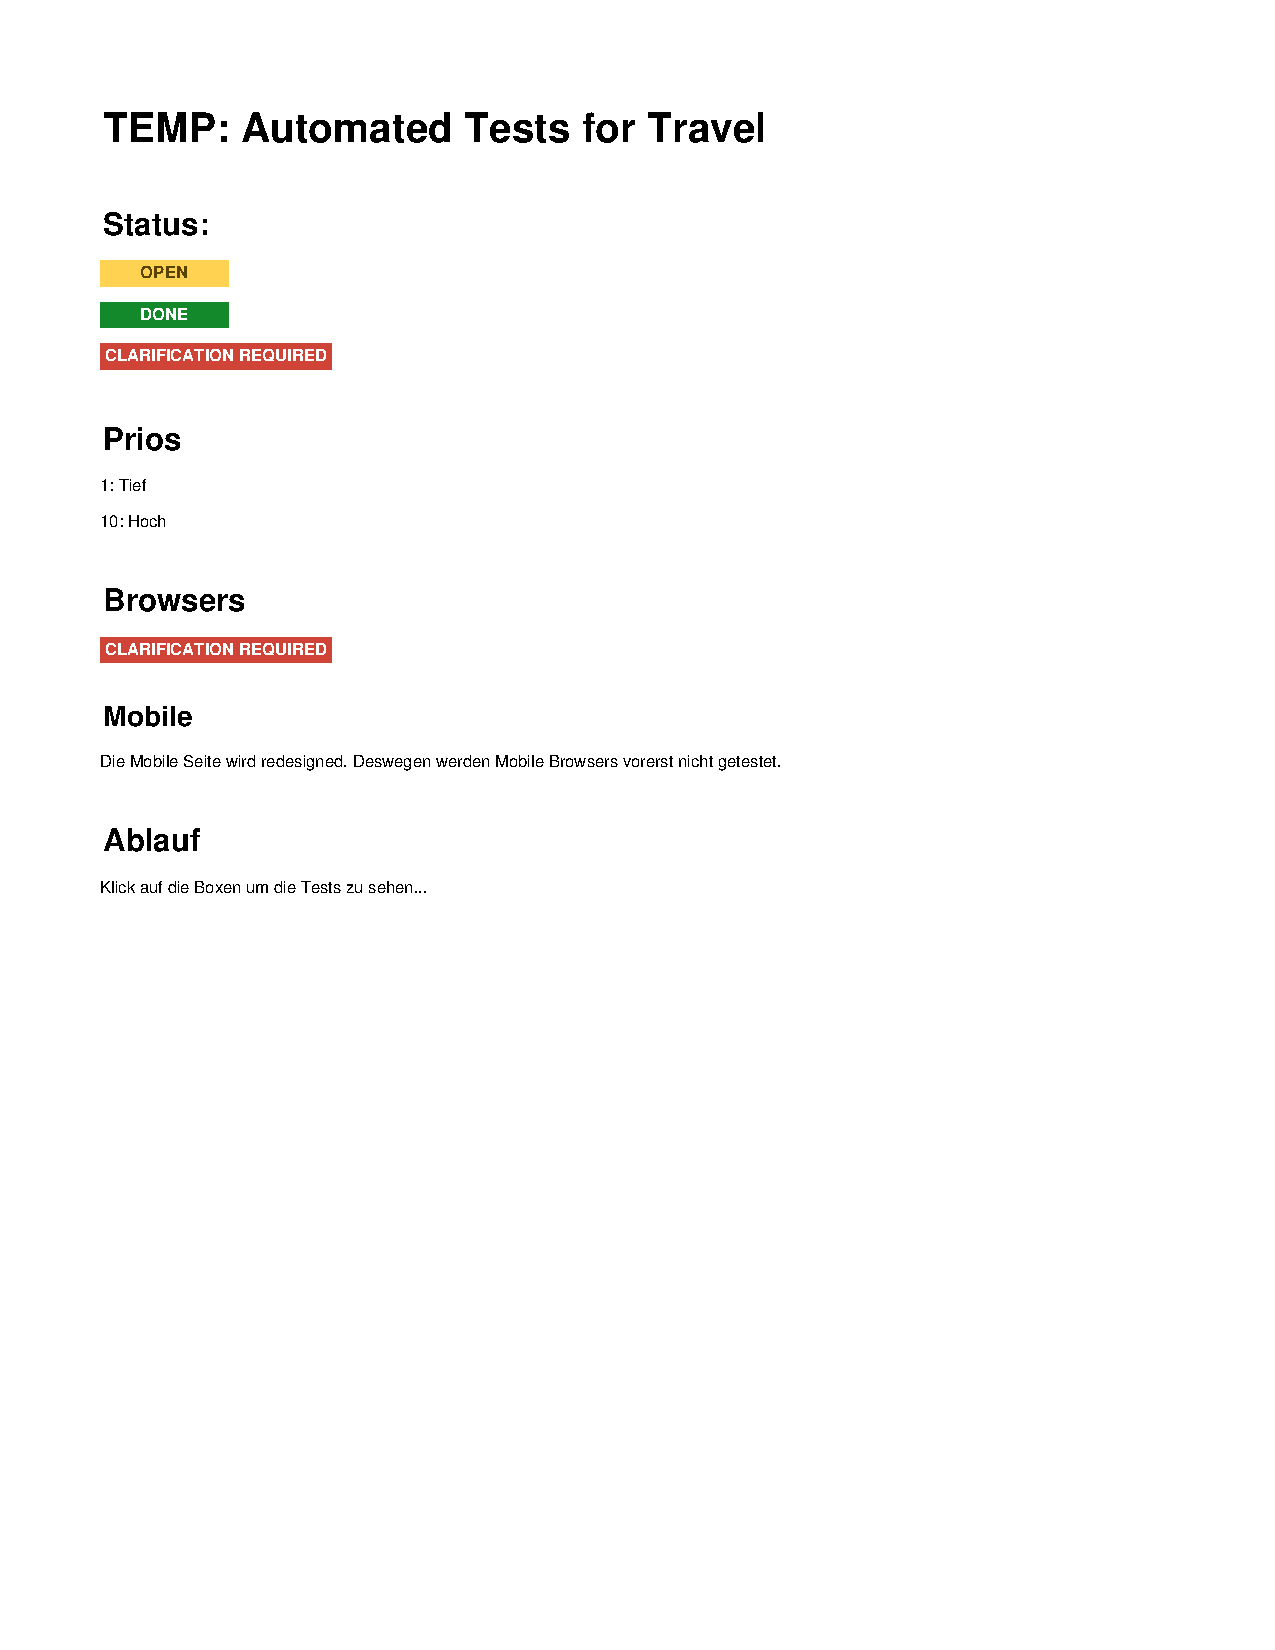
\includepdf[scale=0.8,pages=1,pagecommand=\section{Testübersicht}]{./../test-documentation-1-overview.pdf}
\includepdf[scale=0.8,pages=2,pagecommand=\subsubsection{}]{./../test-documentation-1-overview.pdf}
\includepdf[scale=0.8,pages=3,pagecommand=\subsubsection{}]{./../test-documentation-1-overview.pdf}
\includepdf[scale=0.8,pages=4,pagecommand=\subsubsection{}]{./../test-documentation-1-overview.pdf}
\includepdf[scale=0.8,pages=5,pagecommand=\subsubsection{}]{./../test-documentation-1-overview.pdf}

\chapter{Funktionalitäten}
\label{app:Funktionalitäten}
Folgend ist die gesamte Funktionalität der travel.ch Webseite aufgeführt. Aufgeteilt sind die Funktionalität nach den Webseiten, auf welchen sie angezeigt werden.

Die wichtigsten Felder sind die \textit{Beschreibung}, der \textit{Status} und die \textit{Priorität}. Die Beschreibung erläutert die Funktionalität. Der Status zeigt an, ob eine Funktionalität noch zu testen ist (OPEN), bereits getestet ist (DONE), oder weitere Abklärungen benötigt werden (CLARIFICATION REQUIRED). Die Prioritäten sind in einer Skala von 1 bis 10 angegeben, wobei 10 am dringlichsten ist und 1 am unwichtigsten ist.

Zur Einteilung der Funktionalitäten sind die beiden Felder \textit{Kategorie} und \textit{Engine} vorhanden. Die Spalte "`Notizen"' kann mit einer Frage befüllt werden, wenn der Status auf CLARIFICATION REQUIRED gesetzt ist, oder sonstige Informationen beinhalten. \textit{Implemented in} soll den Entwicklern helfen die Übersicht zu behalten, welche Tests welche Funktionalitäten abdecken.


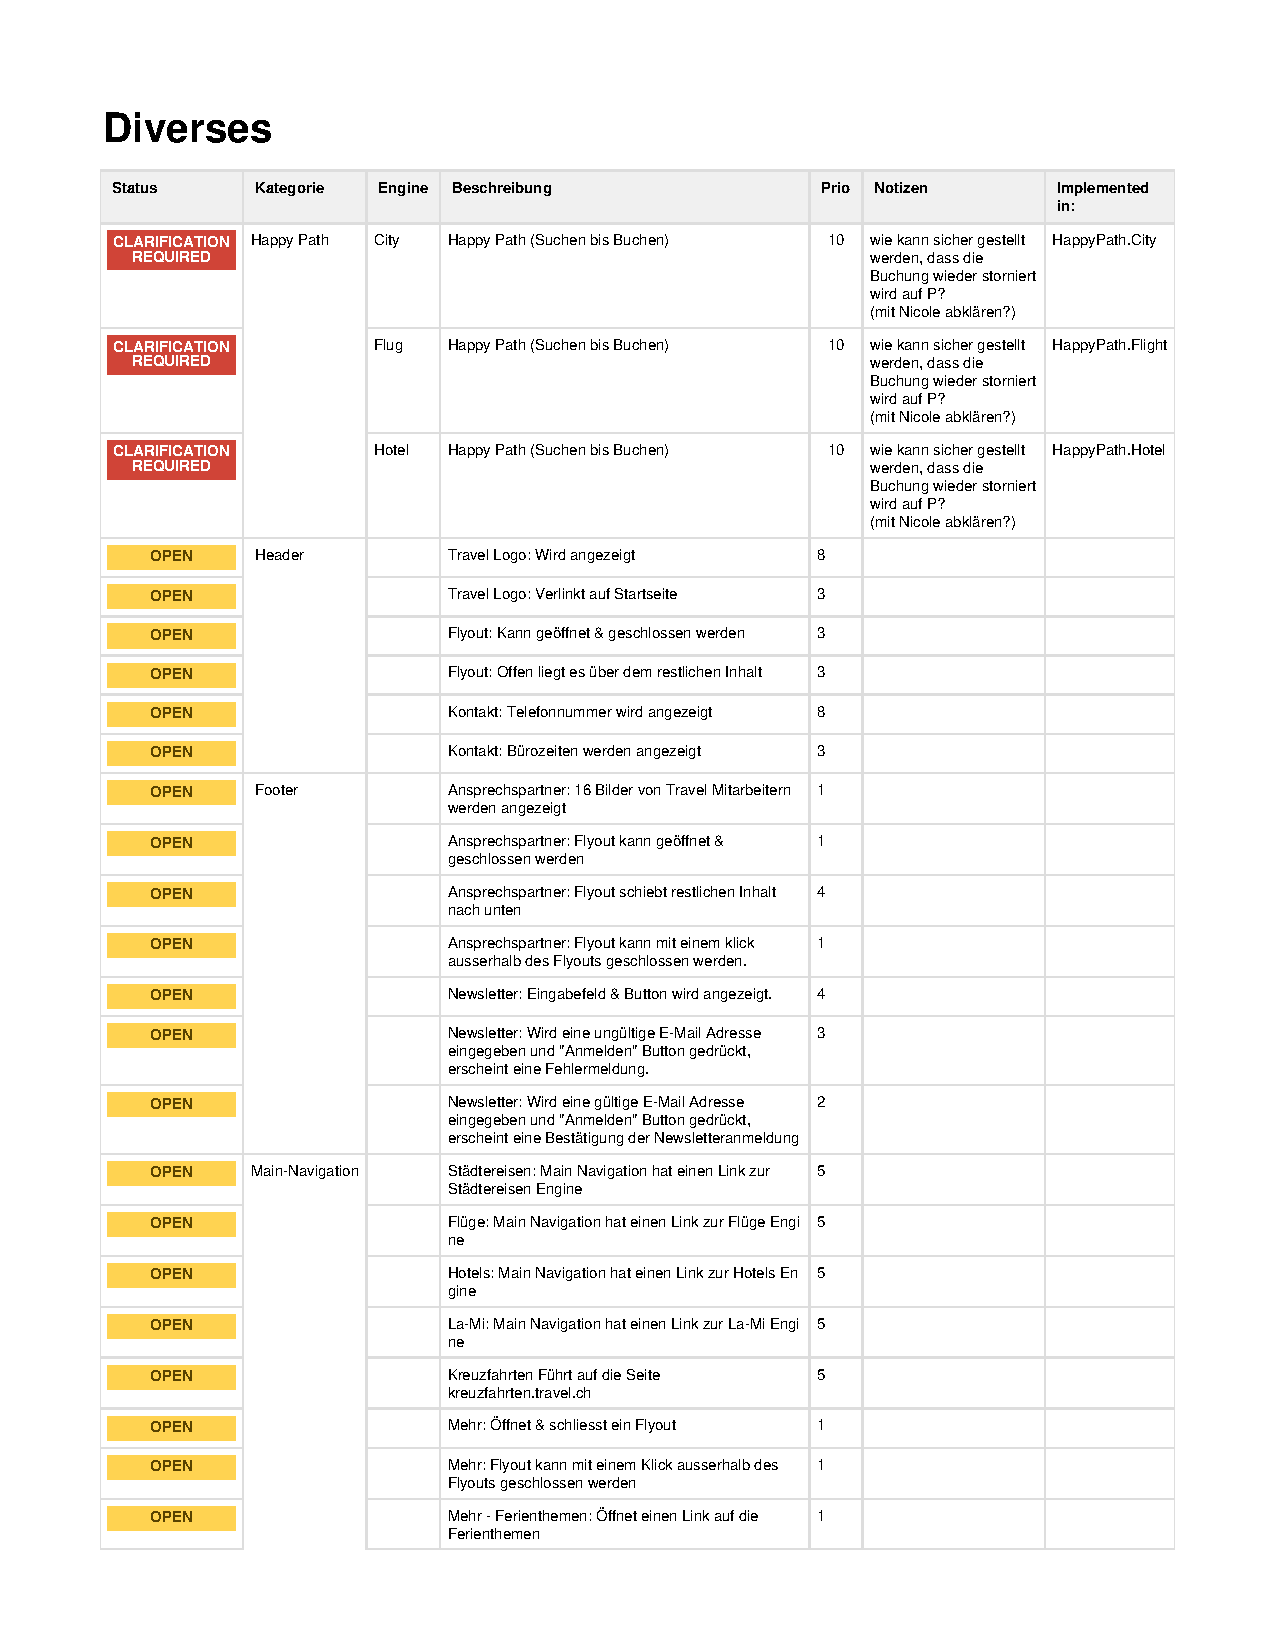
\includepdf[scale=0.8,pages=1,pagecommand=\section{Diverses}]{./../test-documentation-2-miscellaneous.pdf}
\includepdf[scale=0.8,pages=2,pagecommand=\subsubsection{}]{./../test-documentation-2-miscellaneous.pdf}


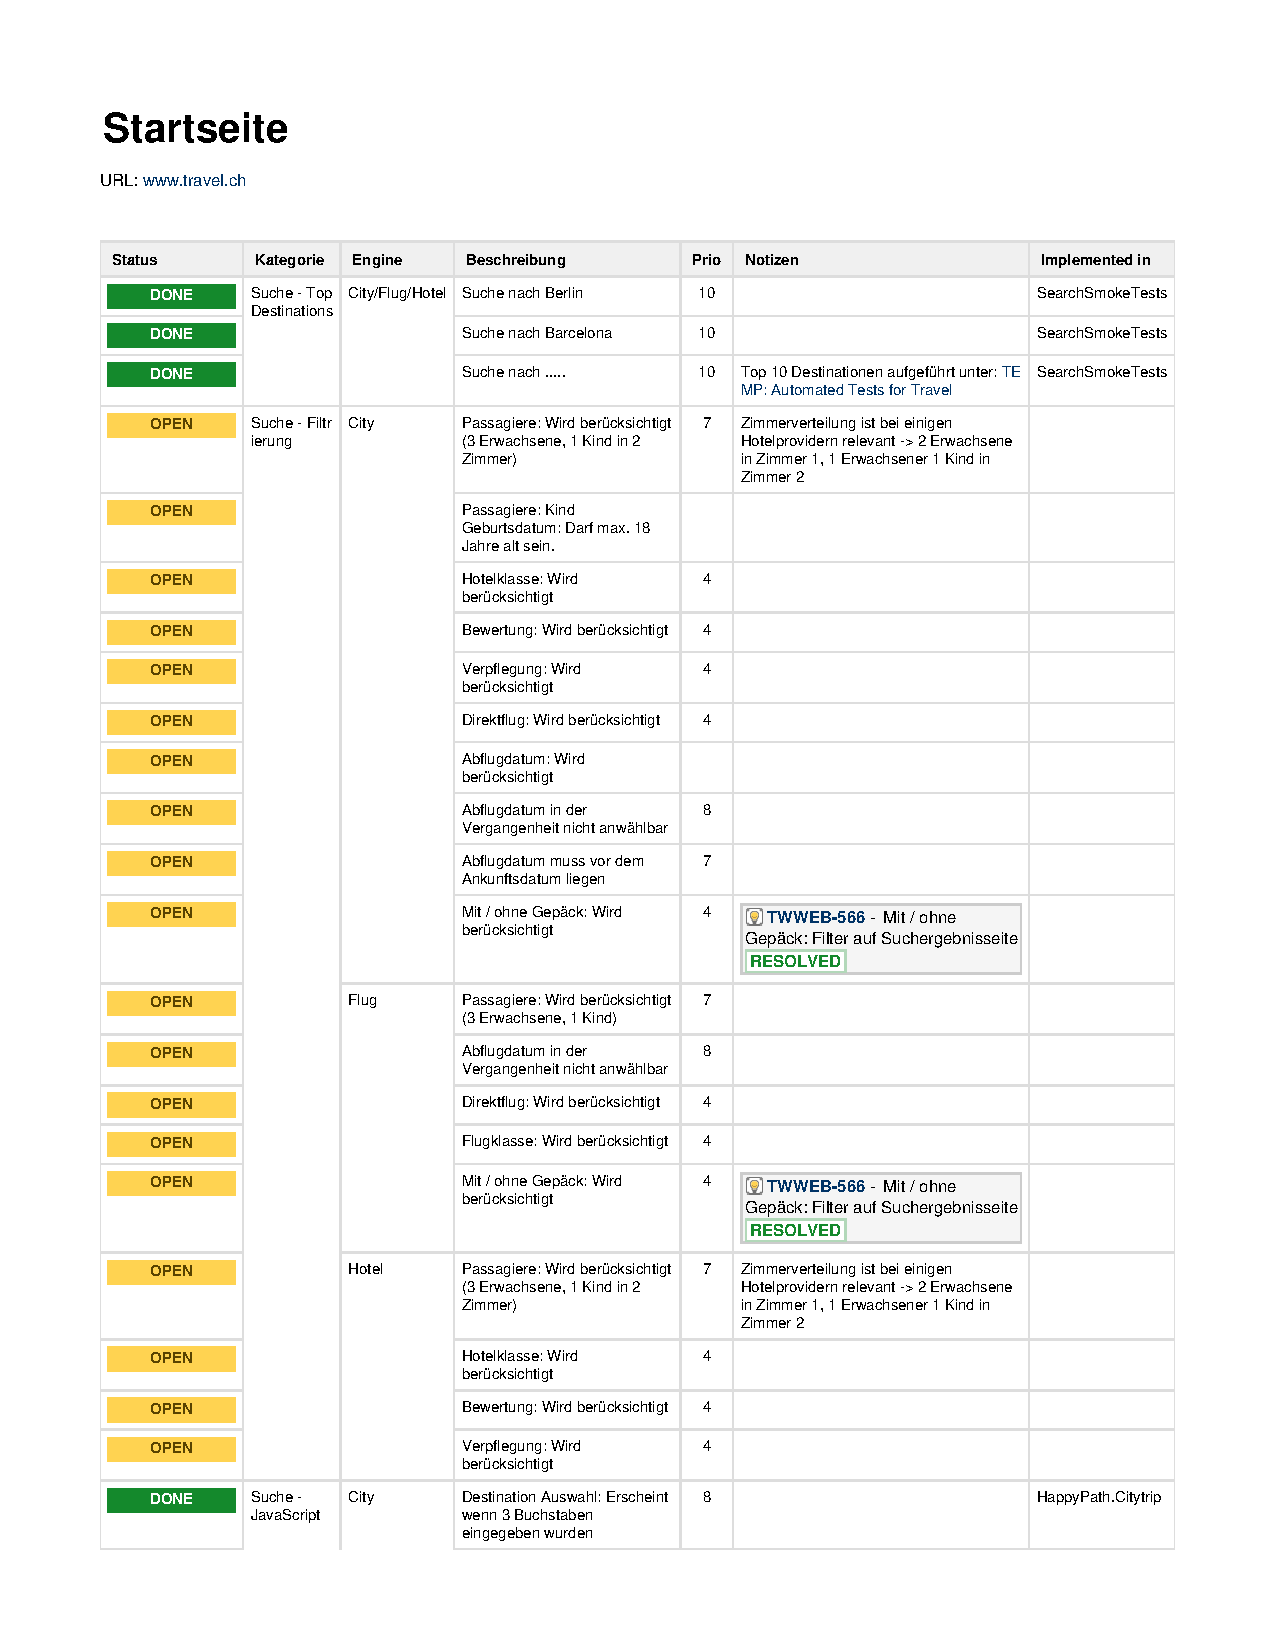
\includepdf[scale=0.8,pages=1,pagecommand=\section{Startseite}]{./../test-documentation-3-startpage.pdf}
\includepdf[scale=0.8,pages=2,pagecommand=\subsubsection{}]{./../test-documentation-3-startpage.pdf}
\includepdf[scale=0.8,pages=3,pagecommand=\subsubsection{}]{./../test-documentation-3-startpage.pdf}
\includepdf[scale=0.8,pages=4,pagecommand=\subsubsection{}]{./../test-documentation-3-startpage.pdf}


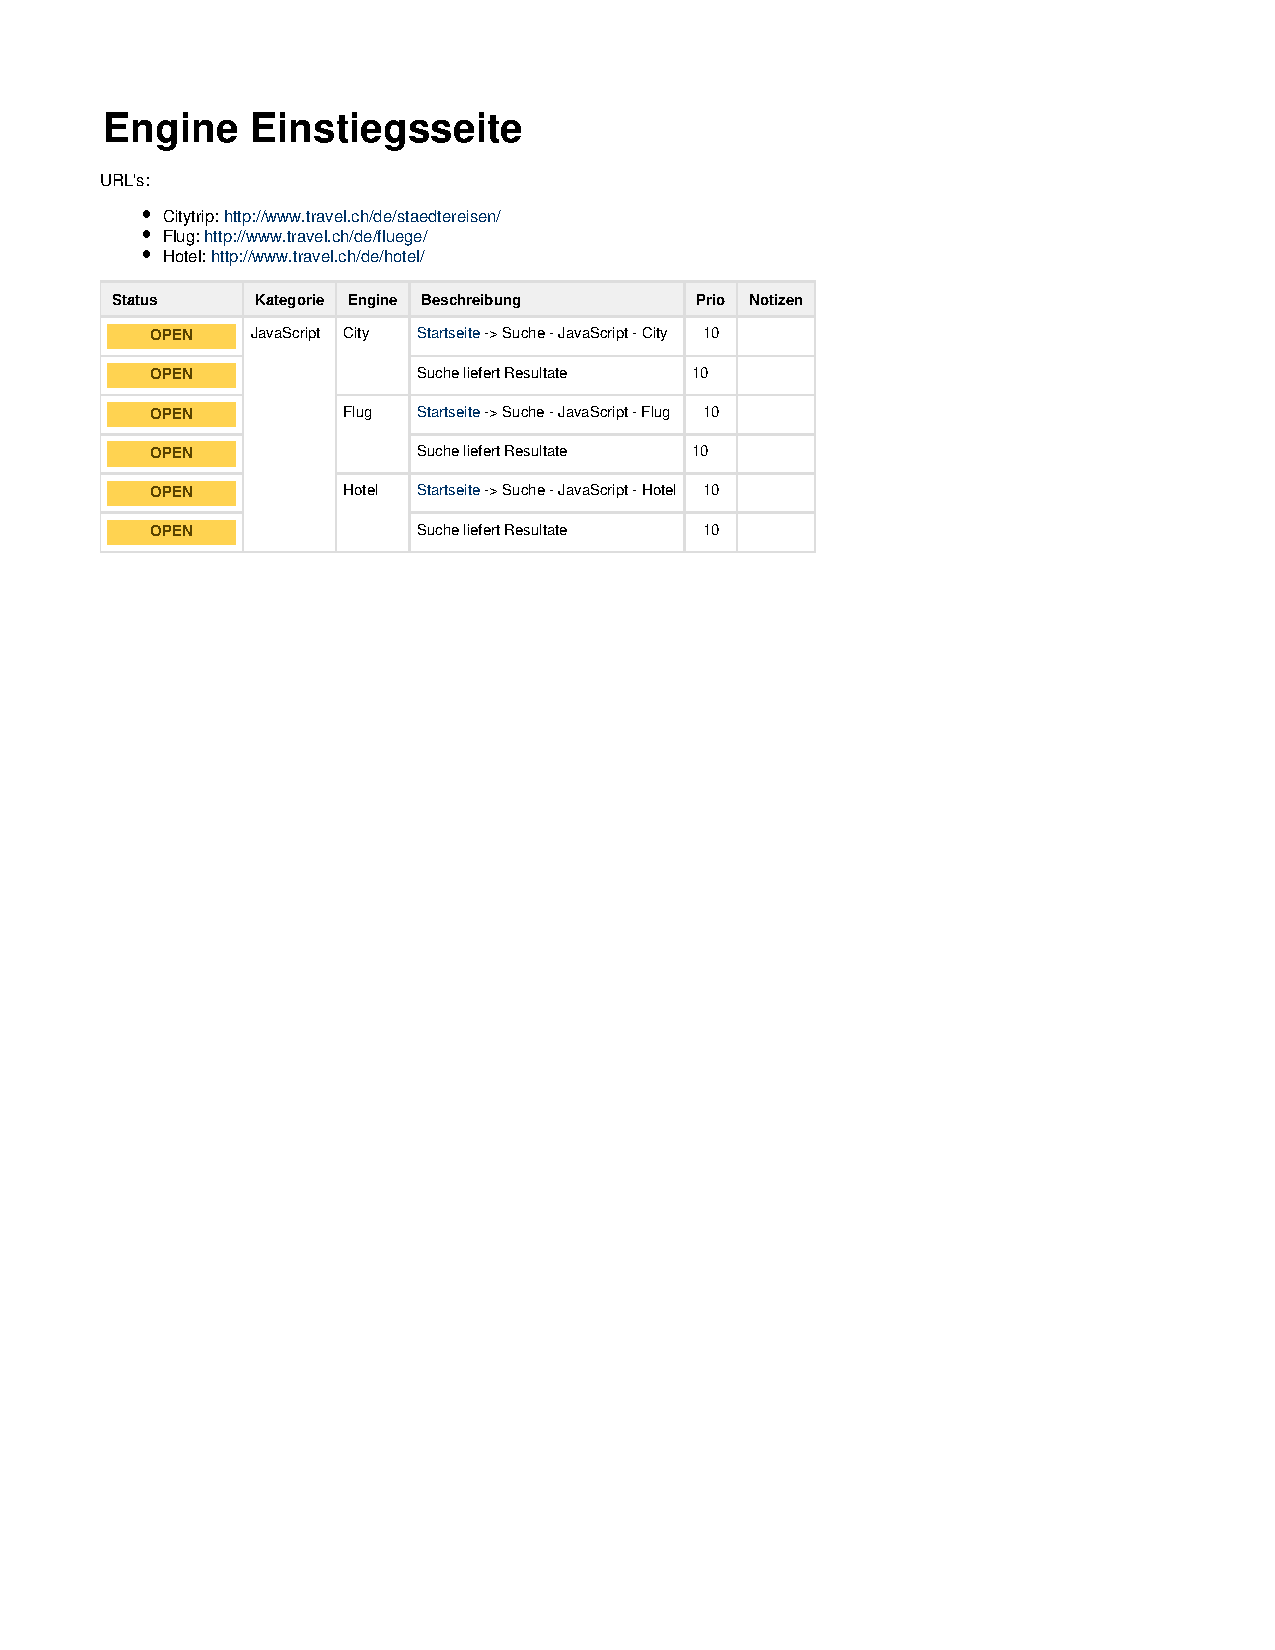
\includepdf[scale=0.8,pages=-,pagecommand=\section{Engine Startseite}]{./../test-documentation-4-engine-startpage.pdf}


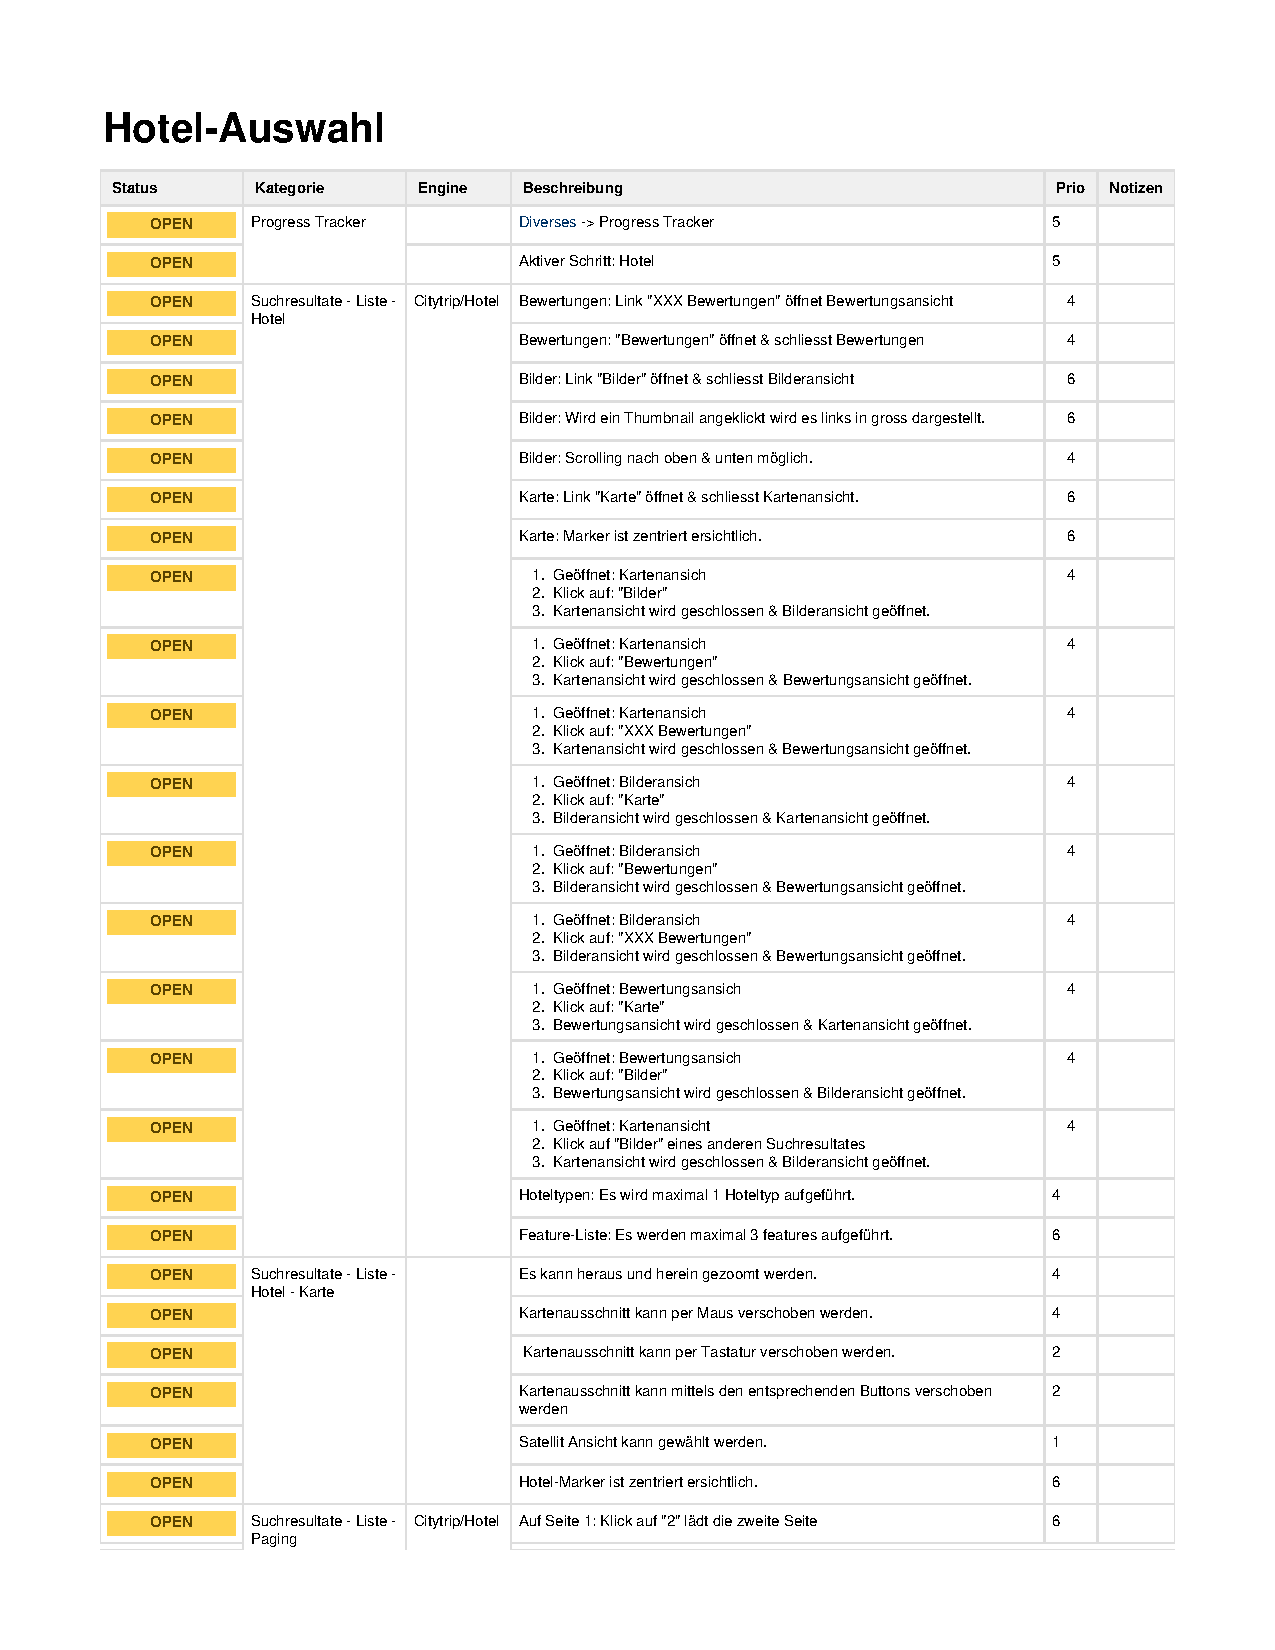
\includepdf[scale=0.8,pages=1,pagecommand=\section{Hotelauswahl}]{./../test-documentation-5-hotel-selection.pdf}
\includepdf[scale=0.8,pages=2,pagecommand=\subsubsection{}]{./../test-documentation-5-hotel-selection.pdf}
\includepdf[scale=0.8,pages=3,pagecommand=\subsubsection{}]{./../test-documentation-5-hotel-selection.pdf}


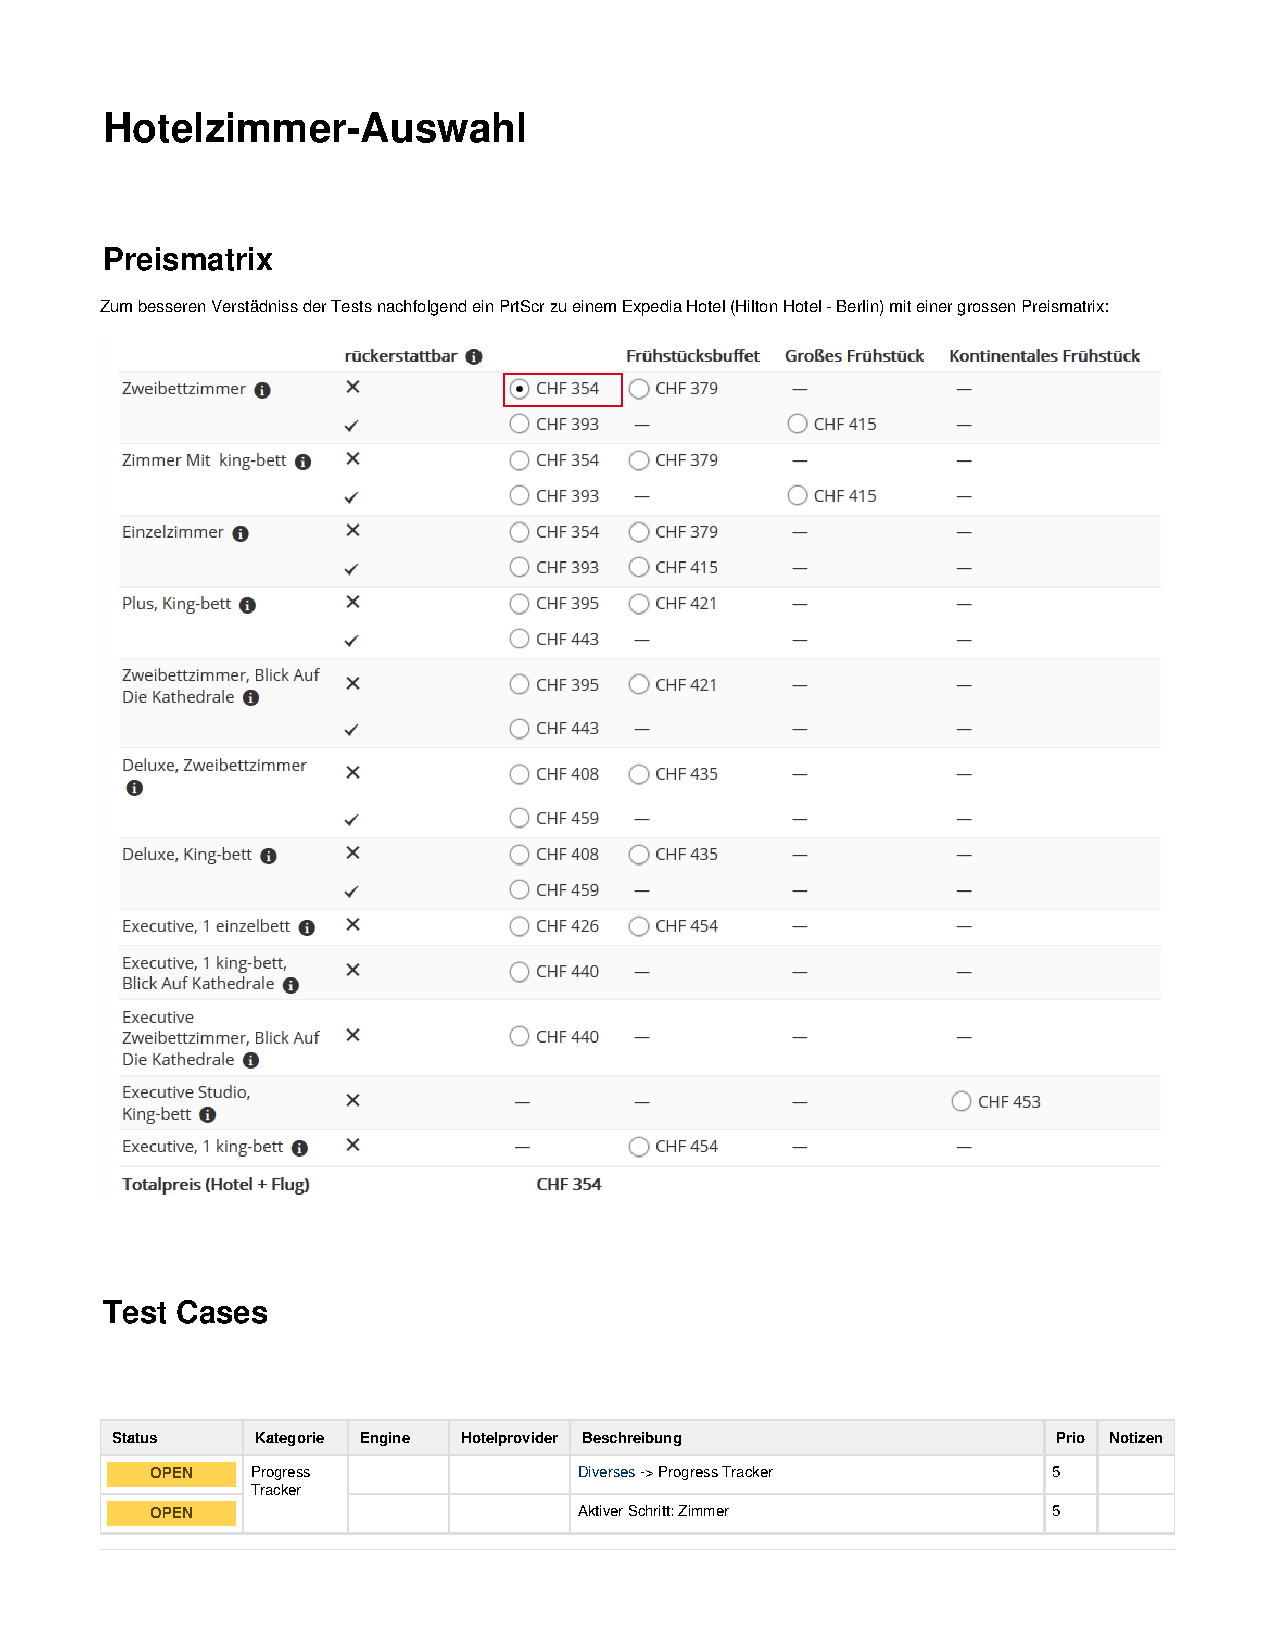
\includepdf[scale=0.8,pages=1,pagecommand=\section{Hotelzimmer Auswahl}]{./../test-documentation-6-hotelroom-selection.pdf}
\includepdf[scale=0.8,pages=2,pagecommand=\subsubsection{}]{./../test-documentation-6-hotelroom-selection.pdf}
\includepdf[scale=0.8,pages=3,pagecommand=\subsubsection{}]{./../test-documentation-6-hotelroom-selection.pdf}


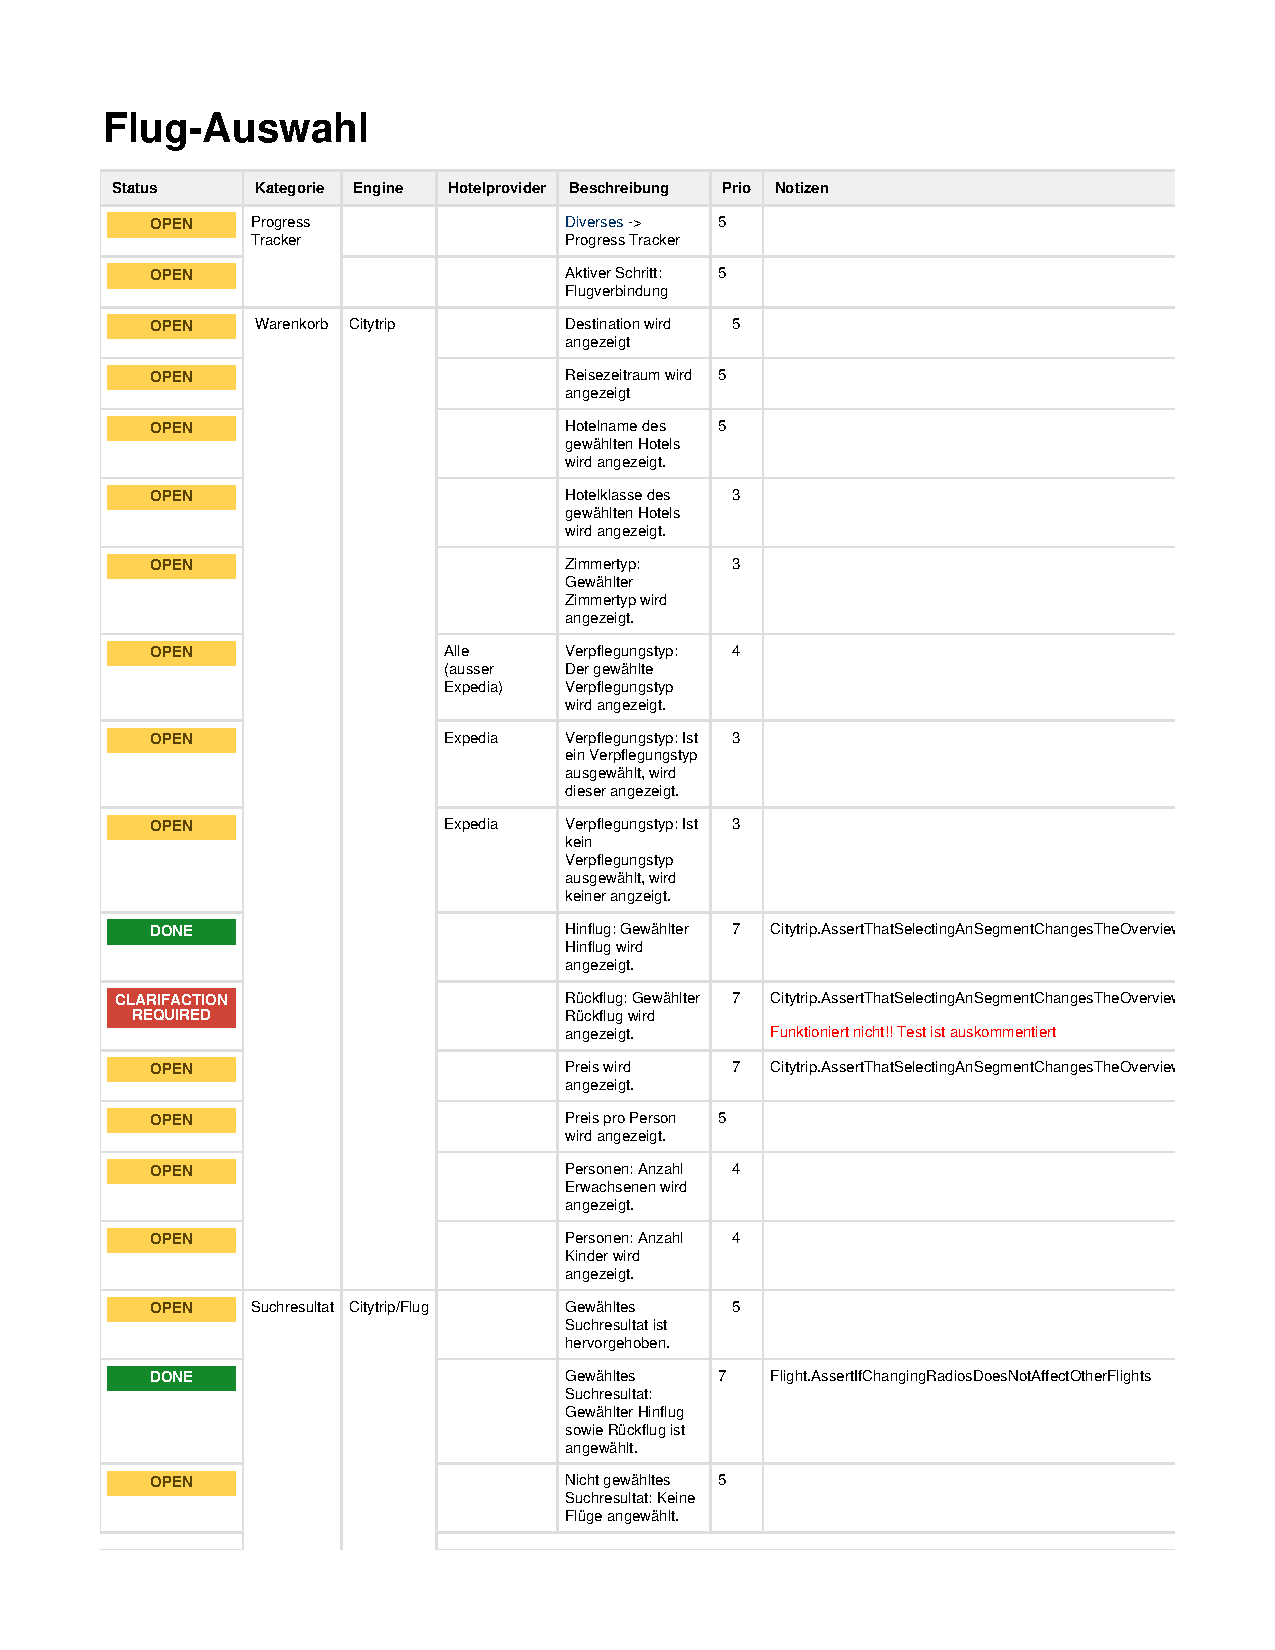
\includepdf[scale=0.8,pages=1,pagecommand=\section{Flugauswahl}]{./../test-documentation-7-flight-selection.pdf}
\includepdf[scale=0.8,pages=2,pagecommand=\subsubsection{}]{./../test-documentation-7-flight-selection.pdf}
\includepdf[scale=0.8,pages=3,pagecommand=\subsubsection{}]{./../test-documentation-7-flight-selection.pdf}


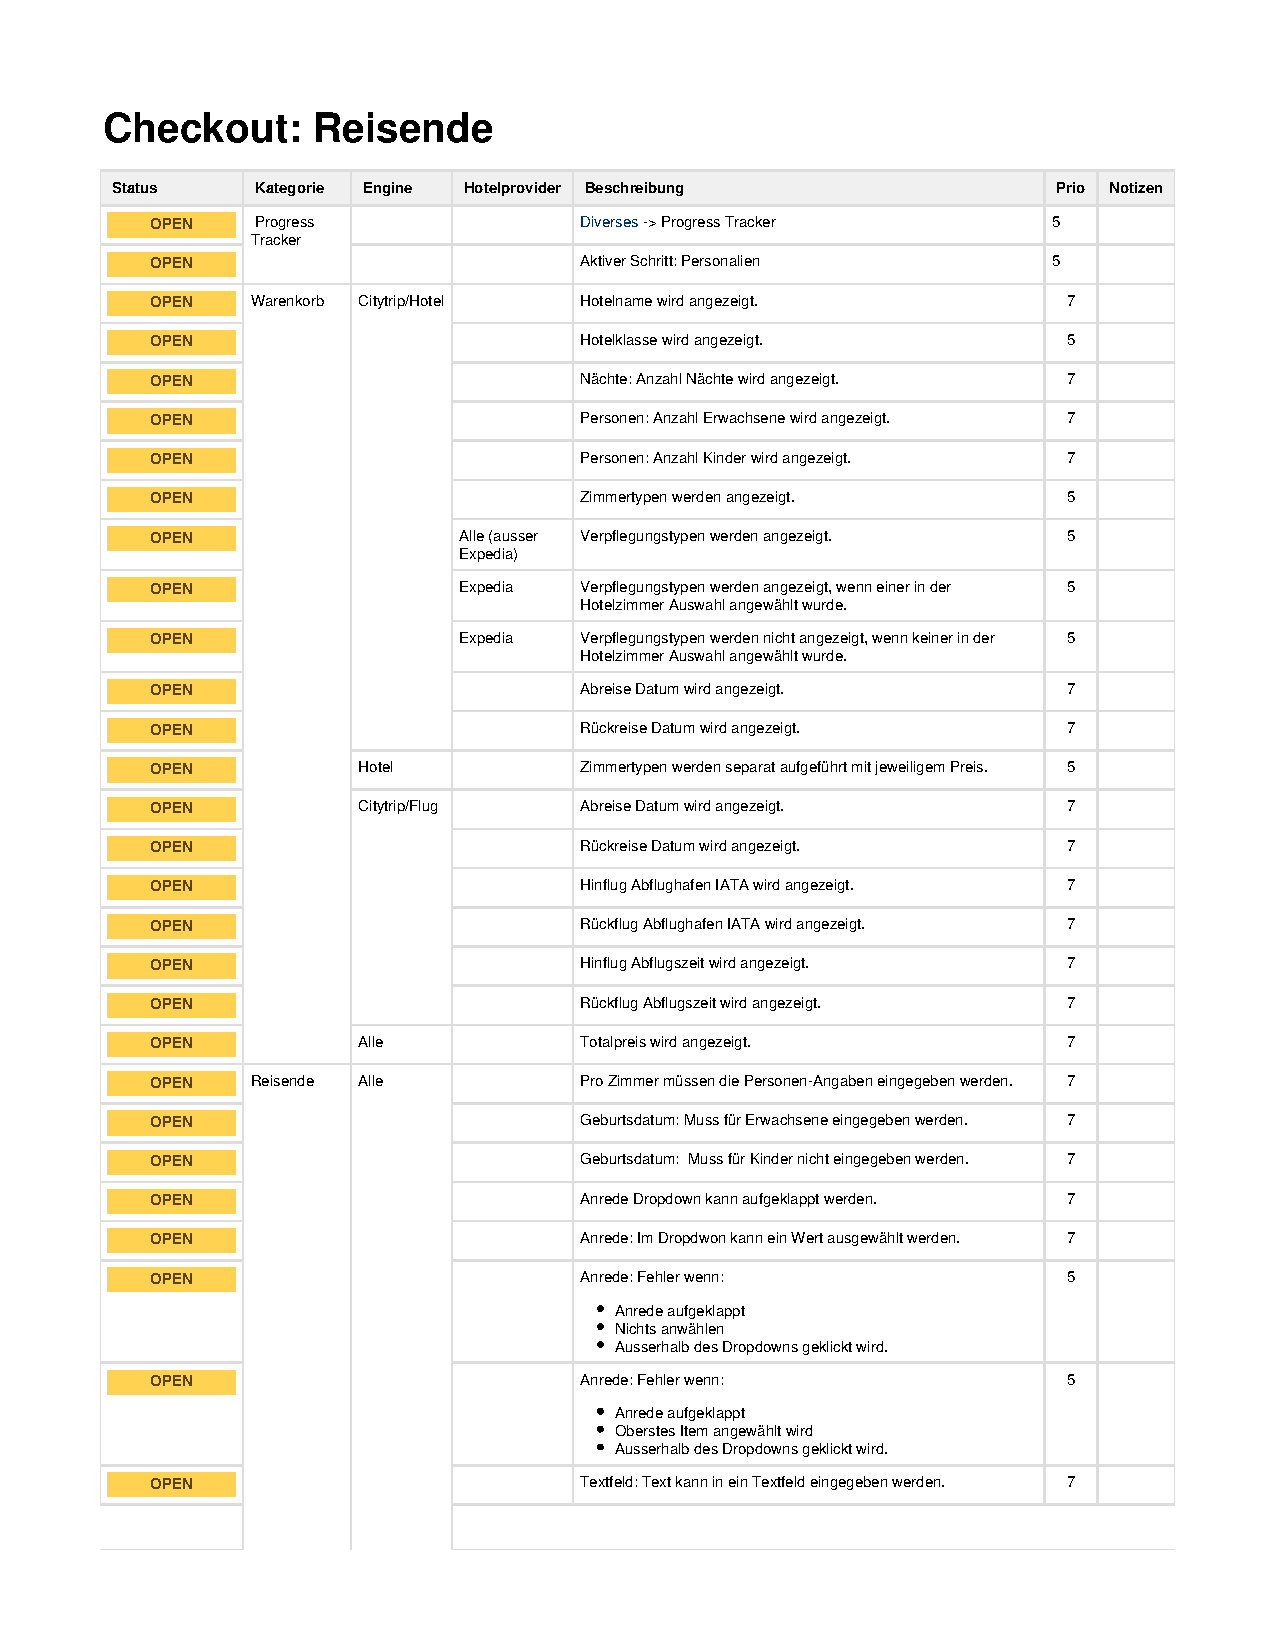
\includepdf[scale=0.8,pages=1,pagecommand=\section{Checkout: Passagiere}]{./../test-documentation-8-checkout-passengers.pdf}
\includepdf[scale=0.8,pages=2,pagecommand=\subsubsection{}]{./../test-documentation-8-checkout-passengers.pdf}


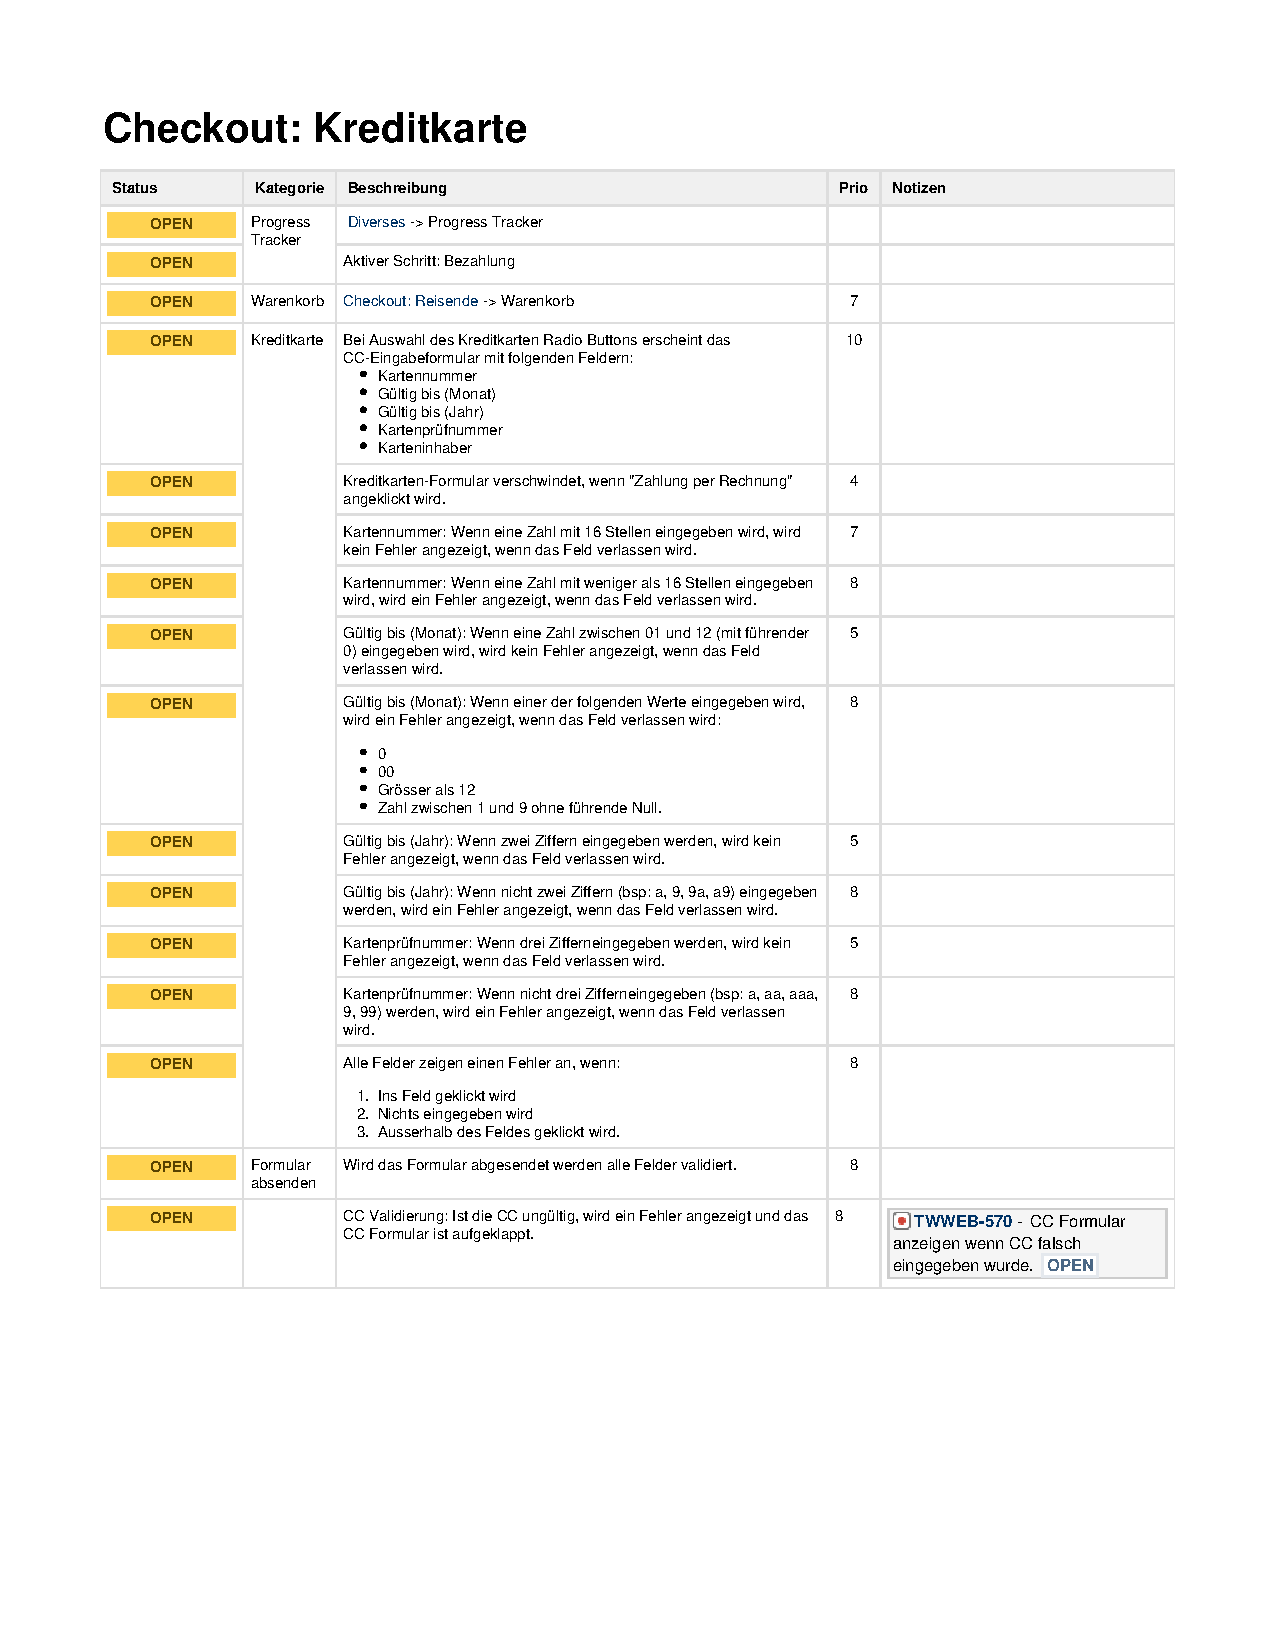
\includepdf[scale=0.8,pages=-,pagecommand=\section{Checkout: Bezahlart}]{./../test-documentation-9-checkout-payment.pdf}


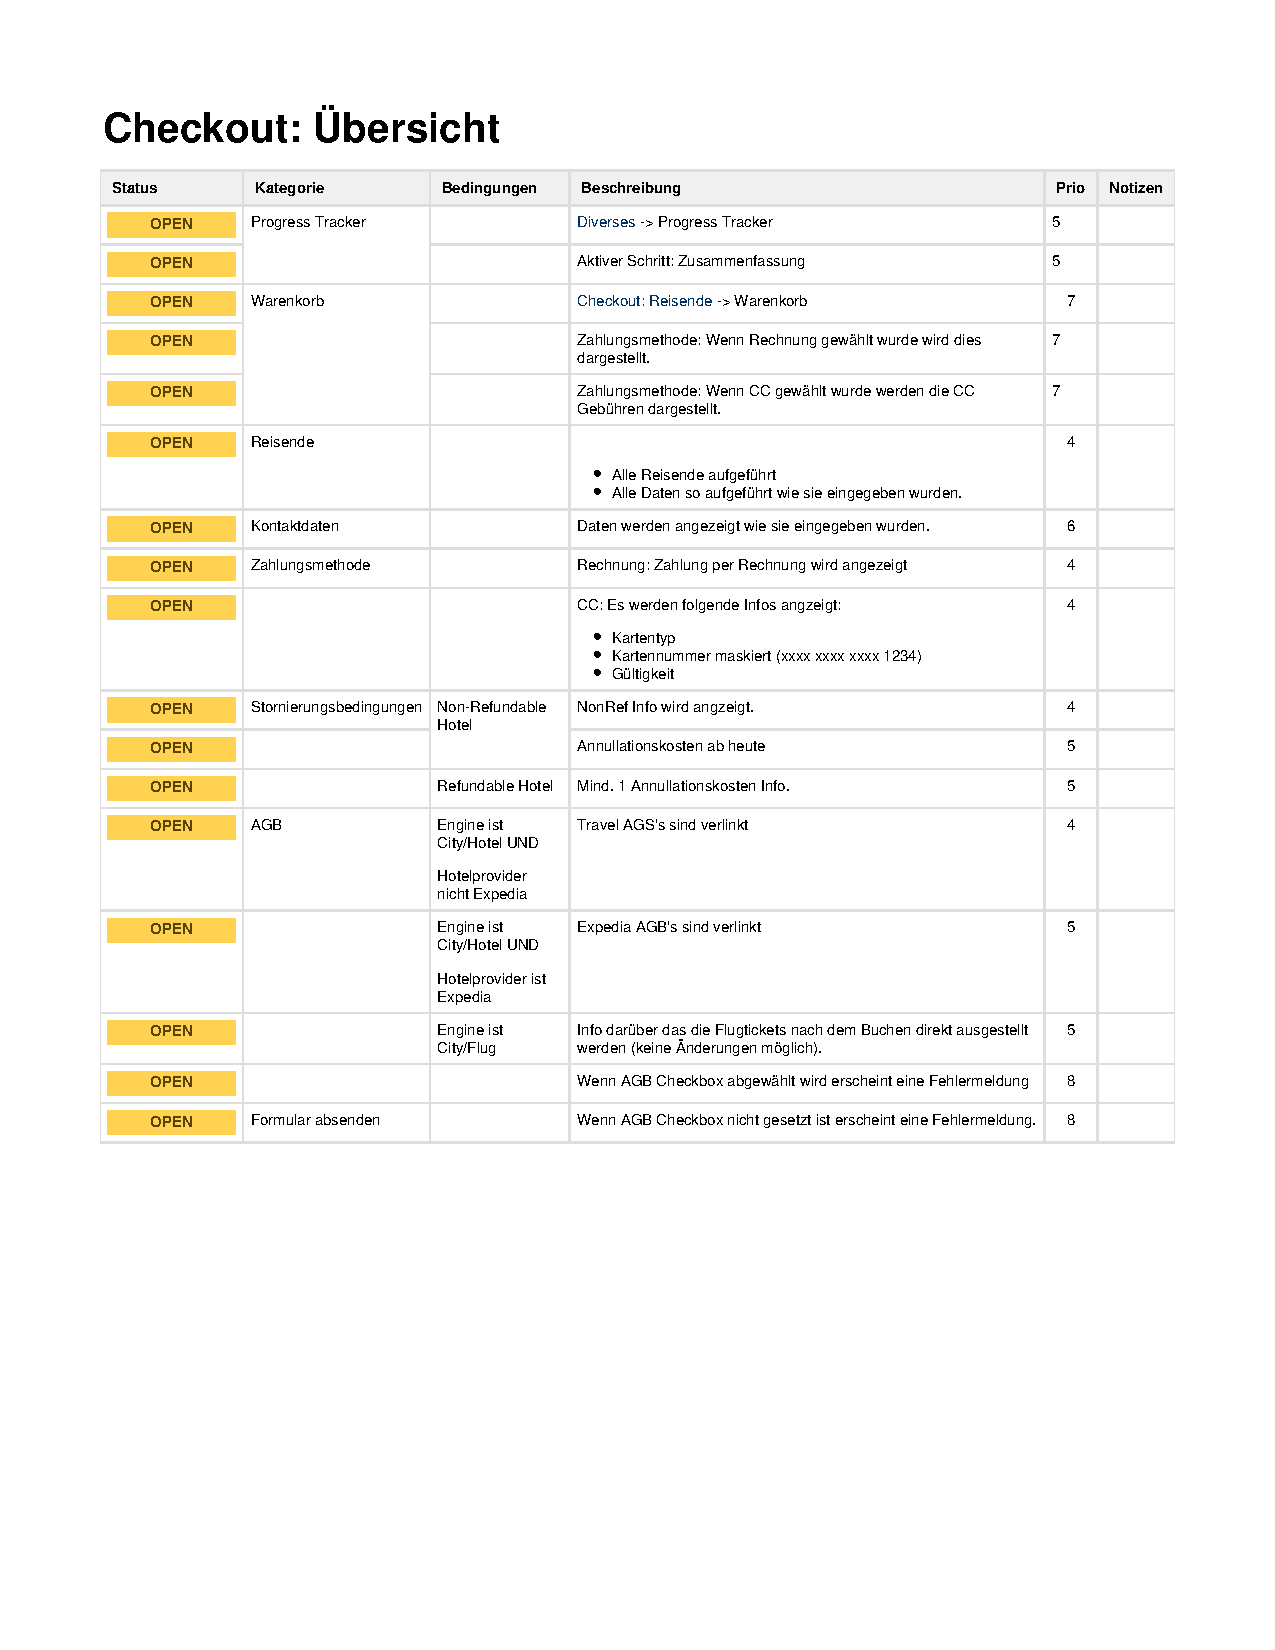
\includepdf[scale=0.8,pages=-,pagecommand=\section{Checkout: Übersicht}]{./../test-documentation-10-checkout-overview.pdf}


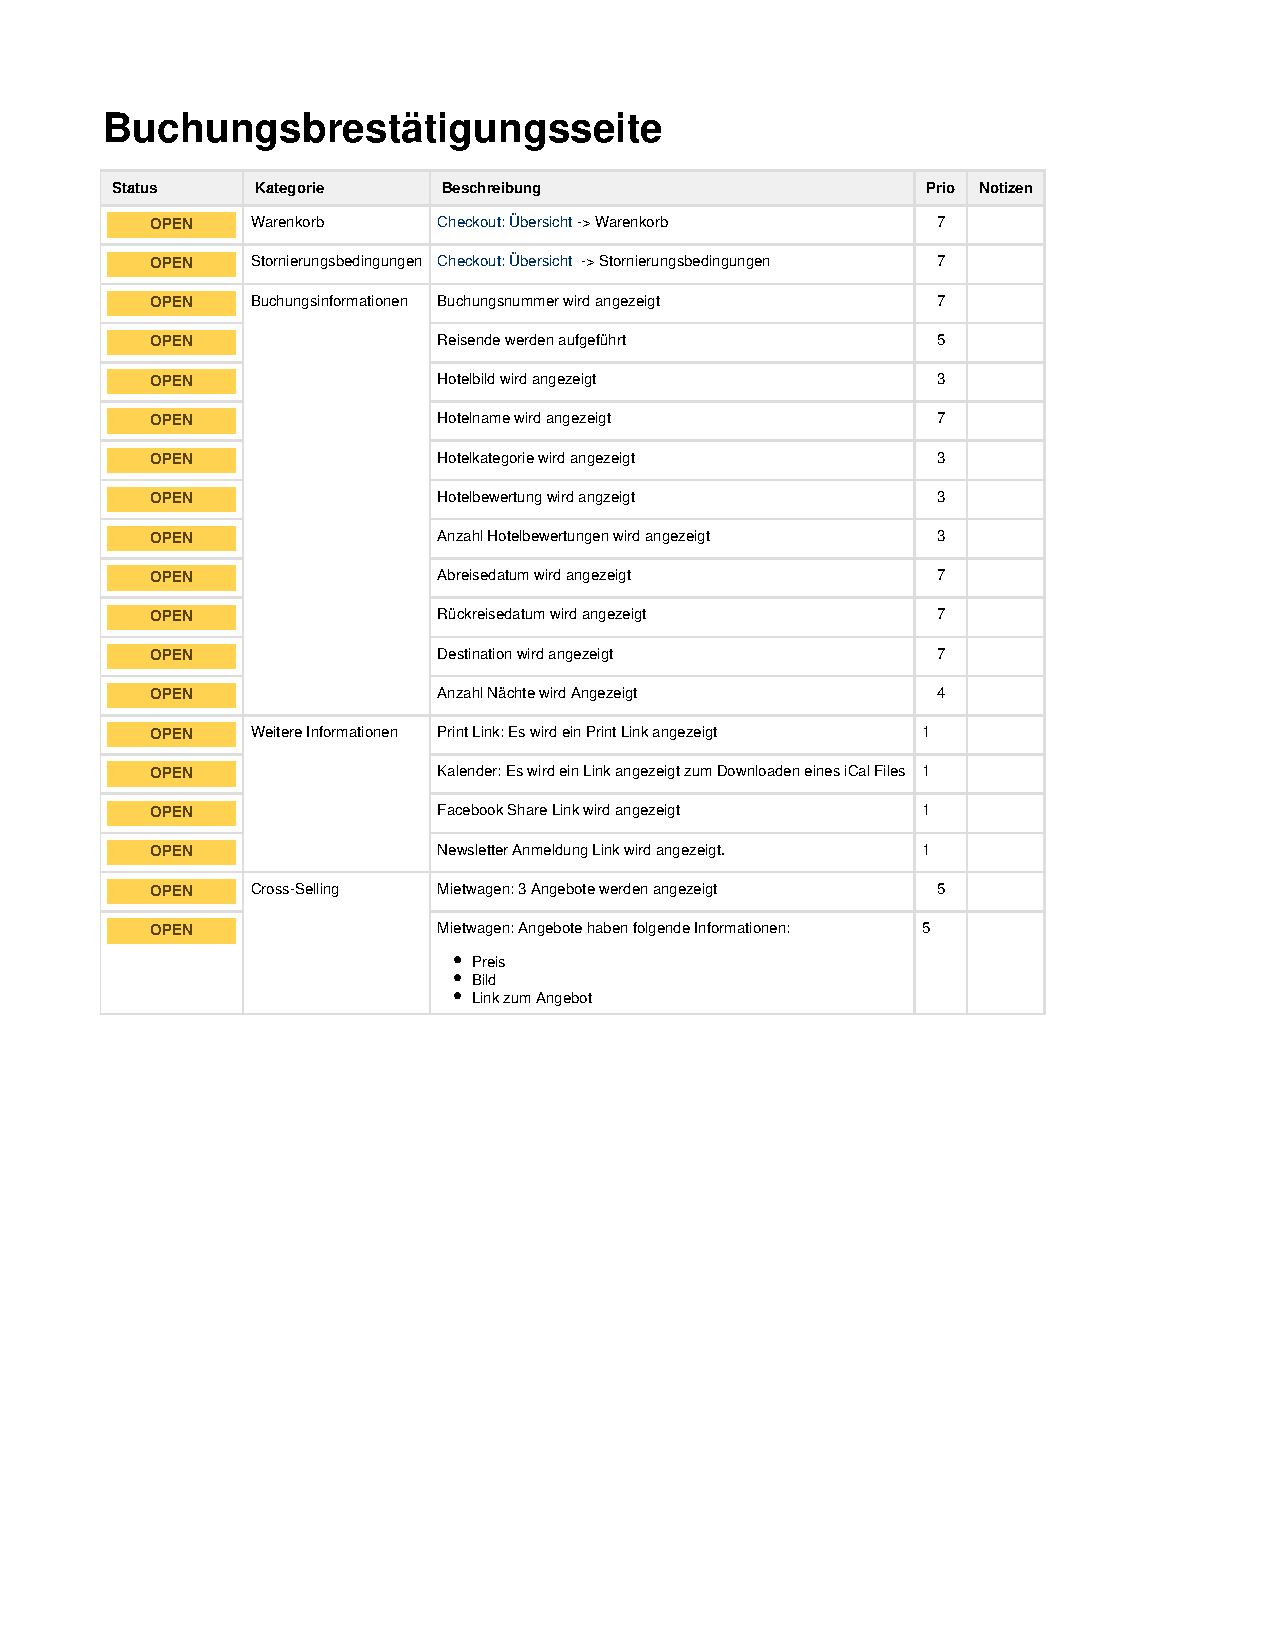
\includepdf[scale=0.8,pages=-,pagecommand=\section{Bestätigungsseite}]{./../test-documentation-11-confirmationpage.pdf}

\chapter{Airlines und Allianzen}
\label{app:airlines}
Die folgenden Listen zeigen alle Airlines und Allianzen auf, welch ein der Suche auf der travel.ch Webseite gewählt werden können (siehe \cref{sec:analyse:grenzwertanalyse} \nameref{sec:analyse:grenzwertanalyse}).
\begin{itemize}
\item Allianzen
	\begin{itemize}
	\item Star Alliance
	\item Oneworld
	\item Skyteam
	\end{itemize}
\item Airlines
	\begin{itemize}
	\item Swiss
	\item British Airways
	\item airberlin
	\item Lufthansa
	\item Delta Air Lines
	\item Iberia
	\item KLM Royal Dutch Airlines
	\item Air France
	\item Singapore Airlines
	\item Austrian Airlines
	\item Emirates
	\item TAP Air Portugal
	\item American Airlines
	\item Turkish Airlines
	\item SAS Scandinavian Airlines
	\item Continental Airlines
	\item Czech Airlines
	\item Thai Airways
	\item United Airlines
	\item Qatar Airways
	\item US Airways
	\item Air Canada
	\item Finnair
	\item Adria Airways
	\item Aegean Airlines
	\item Aer Lingus
	\item Aeroflot
	\item Aerolineas Argentinas
	\item Aerolitoral
	\item Air Algerie
	\item Air Alps Aviation
	\item Air Arabia
	\item Air Arabia
	\item Air Armenia
	\item Air Baltic
	\item Air Botswana
	\item Air Cairo
	\item Air Canada
	\item Air China
	\item Air Dolomiti
	\item Air Europa
	\item Air France
	\item Air Gabon
	\item Air Iceland
	\item Air India
	\item Air Jamaica
	\item Air Madagascar
	\item Air Malta
	\item Air Mauritius
	\item Air Namibia
	\item Air New Zealand
	\item Air Nostrum
	\item Air One Italia
	\item Air Pacific
	\item Air Philippines
	\item Air Plus Comet Argentina
	\item Air Serbia
	\item Air Seychelles
	\item Air Tanzania
	\item Air Transat
	\item Air Ukraine
	\item Air Vanuatu
	\item Air Wales
	\item airberlin
	\item Alaska Airlines
	\item Alitalia
	\item Alitalia CityLiner
	\item All Nippon Airways
	\item Alpi Eagles
	\item America West Airlines
	\item American Airlines
	\item Arkia Israeli Airline
	\item Armavia
	\item Asiana Airlines Inc.
	\item Atlantic Southeast Airlines
	\item Augsburg Airways
	\item Austrian Airlines
	\item Avianca
	\item Aviateca
	\item Azerbaijan Airlines
	\item BA CityFlyer
	\item Bangkok Airways
	\item Belair Airlines AG
	\item Blue 1
	\item Braathens ASA
	\item Britannia  Airways
	\item British Airways
	\item British Midland Regional
	\item Bulgaria Air
	\item CanJet
	\item Cathay Pacific
	\item Cayman Airways
	\item CCM Airlines
	\item China Airlines
	\item China Eastern Airlines
	\item China Southern
	\item CityJet
	\item Comair
	\item Condor
	\item Contact Air
	\item Continental Airlines
	\item Copa
	\item Croatia Airlines
	\item Cubana
	\item Czech Airlines
	\item dba Deutsche BA
	\item Delta Air Lines
	\item Dragonair
	\item Dutch Antilles Express
	\item Easyjet
	\item Edelweiss Air
	\item Egyptair
	\item EL AL
	\item Emirates
	\item Eritrean Airlines
	\item Estonian Air
	\item Ethiopian Airlines
	\item Etihad Airways
	\item Eurowings
	\item Eva Airways
	\item Finnair
	\item Fly Niki
	\item flybe.com
	\item Freebird Air
	\item Garuda Indonesia
	\item Georgian Airways
	\item Germanwings
	\item Gulf Air
	\item Hahn Air
	\item Hawaiian Airlines
	\item Helvetic
	\item HolidayJet
	\item Hop!
	\item Iberia
	\item Iberia Express
	\item Icelandair
	\item Indian Airlines
	\item Intersky
	\item Iran Air
	\item Japan Airlines
	\item Jet Airways INDIA
	\item Kenya Airways
	\item KLM cityhopper
	\item KLM Royal Dutch Airlines
	\item Korean Air
	\item kulula.com
	\item Kuwait Airways
	\item LACSA
	\item Lan Chile
	\item Lan Peru
	\item Lithuanian Airlines
	\item LOT
	\item LTU
	\item Lufthansa
	\item Lufthansa CityLine
	\item Luxair
	\item Malmö Aviation
	\item Martinair
	\item Meridiana
	\item Mexicana
	\item MIAT - Mongolian
	\item Middle East Airlines
	\item Northwest Airlines
	\item Norwegian
	\item Oman Air
	\item OpenSkies
	\item Pakistan Intl. Airlines
	\item Pegasus Airlines
	\item People's Viennaline
	\item Philippine Airlines
	\item Portugalia
	\item Qantas Airways
	\item Qatar Airways
	\item Rossiya
	\item Royal Air Maroc
	\item Royal Brunei
	\item Royal Jordanien
	\item Royal Nepal Airlines
	\item S7 Airlines
	\item SAS Scandinavian Airlines
	\item Saudi Arabian Airlines
	\item SilkAir
	\item Singapore Airlines
	\item Sky Work Airlines
	\item SN Brussels Airlines
	\item South African Airways
	\item Southwest Airlines
	\item SriLankan
	\item Swiss
	\item TACA
	\item TAM
	\item TAM Mercosur
	\item TAP Air Portugal
	\item Tarom
	\item Thai Airways
	\item Transavia
	\item Tunis Air
	\item Turkish Airlines
	\item Tyrolean Airways
	\item Uganda Airlines
	\item Ukraine Int. Airlines
	\item United Airlines
	\item US Airways
	\item Uzbekistan Air
	\item Vietnam Airlines
	\item Virgin Atlantic Airways
	\item Virgin Australia
	\item Virgin Express
	\item Vladivostok Air
	\item Vueling
	\item WestJet
	\item Wideroes Flygselskap
	\item Wind Rose Aviation
	\item Yemen Airways
	\item Zambia Airways
	\end{itemize}
\end{itemize}
%\end{document}